%% This is an example file to show how to use JASA_manu.sty and related 
%% files written by Eric C. Anderson.  It's sort of a fly-by-night endeavor,
%% but I got it to work for me!!


\documentclass[12pt, letter]{article}\usepackage[]{graphicx}\usepackage[]{color}
%% maxwidth is the original width if it is less than linewidth
%% otherwise use linewidth (to make sure the graphics do not exceed the margin)
\makeatletter
\def\maxwidth{ %
  \ifdim\Gin@nat@width>\linewidth
    \linewidth
  \else
    \Gin@nat@width
  \fi
}
\makeatother

\definecolor{fgcolor}{rgb}{0.345, 0.345, 0.345}
\newcommand{\hlnum}[1]{\textcolor[rgb]{0.686,0.059,0.569}{#1}}%
\newcommand{\hlstr}[1]{\textcolor[rgb]{0.192,0.494,0.8}{#1}}%
\newcommand{\hlcom}[1]{\textcolor[rgb]{0.678,0.584,0.686}{\textit{#1}}}%
\newcommand{\hlopt}[1]{\textcolor[rgb]{0,0,0}{#1}}%
\newcommand{\hlstd}[1]{\textcolor[rgb]{0.345,0.345,0.345}{#1}}%
\newcommand{\hlkwa}[1]{\textcolor[rgb]{0.161,0.373,0.58}{\textbf{#1}}}%
\newcommand{\hlkwb}[1]{\textcolor[rgb]{0.69,0.353,0.396}{#1}}%
\newcommand{\hlkwc}[1]{\textcolor[rgb]{0.333,0.667,0.333}{#1}}%
\newcommand{\hlkwd}[1]{\textcolor[rgb]{0.737,0.353,0.396}{\textbf{#1}}}%

\usepackage{framed}
\makeatletter
\newenvironment{kframe}{%
 \def\at@end@of@kframe{}%
 \ifinner\ifhmode%
  \def\at@end@of@kframe{\end{minipage}}%
  \begin{minipage}{\columnwidth}%
 \fi\fi%
 \def\FrameCommand##1{\hskip\@totalleftmargin \hskip-\fboxsep
 \colorbox{shadecolor}{##1}\hskip-\fboxsep
     % There is no \\@totalrightmargin, so:
     \hskip-\linewidth \hskip-\@totalleftmargin \hskip\columnwidth}%
 \MakeFramed {\advance\hsize-\width
   \@totalleftmargin\z@ \linewidth\hsize
   \@setminipage}}%
 {\par\unskip\endMakeFramed%
 \at@end@of@kframe}
\makeatother

\definecolor{shadecolor}{rgb}{.97, .97, .97}
\definecolor{messagecolor}{rgb}{0, 0, 0}
\definecolor{warningcolor}{rgb}{1, 0, 1}
\definecolor{errorcolor}{rgb}{1, 0, 0}
\newenvironment{knitrout}{}{} % an empty environment to be redefined in TeX

\usepackage{alltt}
\usepackage[top=1in, bottom=1in, left=1in, right=1in]{geometry}
\usepackage{graphicx}
\usepackage{float}
\usepackage{amsmath, amssymb, mathtools }
\usepackage{enumerate}
\usepackage{array}
\usepackage{fancyhdr}
\usepackage{verbatim}
\usepackage{color}
\usepackage{pstricks}
\usepackage{eqnarray}
\usepackage{psfrag}
\usepackage{epsfig,epsf}
\usepackage{setspace}
\doublespacing
%% THE NEXT TWO LINES INSERT THE PACKAGES FOR JASA FORMAT:
\usepackage[default]{jasa_harvard}    % 	for formatting citations in text
\usepackage{JABES_manu}


%% CHANGING THE 'AND' IN THE HARVARD BIBLIOGRAPHY PACKAGE TO WHAT IT OUGHT TO BE
\renewcommand{\harvardand}{and}


%% A FEW NEWCOMMANDS FOR THE CONTENT IN THE EXAMPLE
%% NOT CRUCIAL TO THE USE OF JASA_manu.sty
\newcommand{\Dir}{\mathrm{Dir}}
\newcommand{\ceil}[1]{\lceil #1 \rceil}
\newcommand{\thh}{^\mathrm{th}}
\newcommand{\modtwo}{\mathrm{[mod~2]}}
\newcommand{\thetaof}[2]{\theta \langle #1;#2\rangle}
\newcommand{\Mpa}{M_\mathrm{P,A}}
\newcommand{\Ma}{M_\mathrm{A}}
\newcommand{\rjaccept}{\mathcal{A}}



%% Here is a hand-formatted bibliography reference list entry.
%% The command should be included in the NOTE field of the entry in the .bib file
\IfFileExists{upquote.sty}{\usepackage{upquote}}{}
\begin{document}




\title{\bf Detecting Differential Expressed Genes in RNA-Seq Data
Accounting for Nuisance Covariates}
\author{Dan Nettleton  and Yet Nguyen\\
Department of Statistics, 
Iowa State University, Ames, IA 50010%\\ 
%email: \texttt{ntyet@iastate.edu}
}

\maketitle


%% ABSTRACT

%\newpage
\begin{center}
\textbf{Abstract}
\end{center}
Differential Expression Analysis of RNA-Seq data can often be complicated by the presence of nuisance factors that arise due to experimental design limitations and heterogeneity of experimental units that can be seen in continuous and categorical covariates measured for each experimental unit and/or RNA sample. The analysis is typically done by including or ignoring all nuisance covariates. Some drawbacks of those approaches are that the FDR usually too conservative or too liberal, and the power of detecting differentiallly expressed genes is very low. To address these shortcoming, we develop a backward selection procedure to pick up the most significant covariates, which inturn are used to identify  genes that are differentially expressed. The proposed method is then applied to RNA-Seq data from Residual Feed Intake project. Furthermore, simulation results from real data show that our proposed method outperforms the traditional strategies used to detect differential expression genes accounting for nuisance covariates.



\vspace*{.3in}

\noindent\textsc{Keywords}: {Backward Model Selection, Grenander Estimator,  False Discovery Rate, Partial AUC, Cramer Von Mises, RNA-Seq, Nuisance Covariates, Differential Expression Analysis.}

%\newpage

\section{\bf Introduction}
A nuisance variable, or confounded variable, is an unwanted variable that is correlated with the outcome within an experimental study and is typically of no interest to the researcher. It might be a characteristic of the experimental unit under study or any unintended influence on an experimental manipulation. A nuisance variable causes greater variability in the distribution of a sample's scores and affects all the groups measured within a given sample. In the situation of RNA-Seq experiment, accounting for nuisance variable is becoming increasingly important due to very expensive cost of the high throughput sequencing technology.

As a specific motivation example, consider the RNA-Seq experiment conducted by ISU  researchers to examine gene expression in two Yorkshire residual feed intake (RFI) pig \emph{lines} feeded either by \emph{high fiber-low energy diet} or \emph{low fiber-high energy diet}. Illumina RNASeq was used to measure gene expression total 31 pigs  of full 2-factor factorial design $\emph{Line} \times \emph{Diet}$. 

The main purpose of the experiment  can be describled as follows. Prior of the experiment, it was known that feed is the largest cost of US pork producer, representing 55 to 60 \% of the total cost. Hence, knowlegde on efficiency of nutrient utilization and development of new technology and mechanisms for improving feed efficiency (FE) is critical to the long term competitiveness of the US pork industry and for improving the sustainability of food supplies. In constrast to the mechanisms that govern  growth and development, our understandingn of the biological mechanisms regulating feed efficienty is limited. Therefore there is a critical need to define the mechanisms that regulate feed efficiency. Koch et. al(?) suggested the concept of residual feed intake to measure FE in cattle. RFI partitions feed intake into two part: the level of intake expected in onder to support a given rate of gain, plus a residual portion. Efficient animals have a low negative RFI, i.e., they consume less feed than expected for their rate of gain. RFI is the unique measure of FE because it represents true differences in the ability of animals to use feed energy for the metabolic processes of maintenance and growth. However, measuring RFI is expensive and time-consuming. The purpose of the study is to use whole blood from 4-5 week-old pigs  to identify differentially expressed genes between two Yorkshire lines of pigs divergently based on RFI, with the final goal of developing usefull biomakers for FE. 

Blood samples were collected into Tempus 
tubes for long-term storage and EDTA tubes for 
complete blood count (CBC) test from 233 piglets 
(Generation 9, at 35 ~ 42 days of age) of the two 
Yorkshire lines of pigs divergently selected for FE 
based on RFI, the low RFI line and the high RFI line. 
We subsequently measured the complete blood count 
(CBC) of all blood samples. These animals were later 
randomly assigned to two diets of different fiber and 
energy content, and each pig’s RFI was measured on 
FIRE feeders. Blood samples of 8 animals of 
extremely low RFI for the low RFI line and 
extremely high RFI for the high RFI line on each diet 
were selected for RNA-sequencing, with one sample 
later dropped due to low RNA quality. RNA samples 
were prepared and globin transcripts were depleted 
by an RNase H-mediated method before RNA 
sequencing. One hundred bp paired-end sequencing 
was run on the Illumina HiSeq 2000 platform. Reads 
were mapped to the pig reference genome 
(Sscrofa10.2.76) using aligner STAR after quality 
trimming and featureCounts was used to get read 
counts for each gene. In summary, the main effect of interest is RFI Line effect (Line), and a number of nuisance covariates such as Diet, RFI value, 
CBC values (lymphocite, neutrophil, monocyte, basophil and eisophil), and some technical variables such as processing batch (Block), processing order (Blockorder), RNA concentration before and after globin depletion (Concb, Conca), RNA Integrity Number before and after globin depletion (RINb, RINa). The RNA-Seq data consists of 12280 genes and 31 samples. 
The preliminary analysis result of this data is either including all nuisance covariates, or ignore all nuisance covariates using QuasiSeq (Lund et al. 2012). There are 2 genes declared differentially expressed between 2 RFI lines if fitting the full model with all covariates when controlling FDR at 5\%.  For the model ignoring all nuicanse covariates, there are 233 differentially expressed genes when controlling FDR at 5\%.   The Figure 1  is showing histograms of pvalues for testing the significant of Line effect for those two scenariors. 
\begin{knitrout}
\definecolor{shadecolor}{rgb}{0.969, 0.969, 0.969}\color{fgcolor}\begin{figure}[H]


{\centering \includegraphics[width=6cm,height=6cm]{figure/minimal-unnamed-chunk-11} 
\includegraphics[width=6cm,height=6cm]{figure/minimal-unnamed-chunk-12} 

}

\caption[The left Figure is the histogram of pvalue of Line effect for model including Line effect and all nuisance covariates]{The left Figure is the histogram of pvalue of Line effect for model including Line effect and all nuisance covariates. The right Figure is the histofram of pvalue of line effect for model including only Line Effect, and does not include any nuisance covariates.\label{fig:unnamed-chunk-1}}
\end{figure}


\end{knitrout}

This article focuses on backward model selection procedure for choosing the model which optimal for differential expression analysis in the sense that the power of detecting differential expression genes is largest. The basis method is described in Section 2. Section 2.1 contains preliminary setup of probability model for RNA-Seq count data. Section 2.2 reviews the results on Grenander estimator of non-increasing probablility distribution function and Kolmogorov-Smirnov statistic between two distribution (ks). Section 2.3 and 2.4 contains the description of backward selection procedure using ks criteria and number of pvalues less than 0.05 (pvalue05), respectively. Section 3 demonstrate the approach using RFI RNA-Seq data above. Section 4 devotes to a simulation study that compares the proposed approach to the traditional approaches which are including or excluding all nuisance covariates. The article concludes and provides ideas for future works in Section 5. 
\section{\bf Methods}
\subsection{\bf Model for Count Data}
Let $y_{ijk}$ is the count of gene $g$ from sample $j$ of treatment group $i$. Then suppose 
\[
y_{gij} \sim NB(\mu_{gij}, \omega_g), \log(\mu_{gij}) = o_{ij} + Line*\beta_{line} + X_{(ij)}\beta,
\]

where $X$ is the desing matrix $31\times 23$ and $X_{(ij)}$ is the row of $X$ 
corresponding to sample $j$ of treatment group $i$, $\beta$ is the vector of parameter corresponding to  nuisance covariates.
\subsection{\bf False Discovery Rate}
...............
\subsection{\bf Grenander Estimator of Non increasing PDF}
The Grenander (1956) density estimator is given by the slopes of the least concave majorant (LCM) of the empirical distribution function (ECDF). It is a decreasing piecewise-constant function and can be shown to be the non-parametric maximum likelihood estimate (NPMLE) under the assumption of a decreasing density (note that the ECDF is the NPMLE without this assumption). 

\subsection{\bf Anderson-Darling Statistics}
The Anderson-Darling  statistics is a criterion used for calculating the distance between  a cumulative distribution function $F^*$ compared to a given empirical distribution function $F_n$, or for comparing two empirical distributions. It is defined as

\[
\omega^2 = \int_{-\infty}^{\infty} [F_n(x)-F^*(x)]^2\,\mathrm{d}F^*(x) .
\]
.....................
\subsection{Backward Selection Procedure and Stopping Criteria}

Starting model includes all covariates of interest. For each covariate,
we conduct a Likelihood Ratio Test using QuasiSeq of the full model
vs. the reduced model obtained from the full model by deleting the
considered covariate. We collect the set of pvalues of all genes from
the tests.
Obtain the number of genes with pvalues less than or equal 0.05 (This is the criterion named pvalue05).
Obtain Grenander CDF estimator of the empirical CDF of the sample
from those pvalues.
Obtain Craḿer-Von-Mises statistics,
 statistics between the Grenander CDF and
uniform(0,1) CDF.
Exclude the covariate corresponding to the smallest value in each criterion.

The procedure will be terminated until the Line effect is excluded.  Then the final model will be used for differential expression analysis will be the model which has largest number of pvalue of Line effect less than 0.05.
\section{\bf Real Data Analysis}
\begin{figure}[h!]
\centering
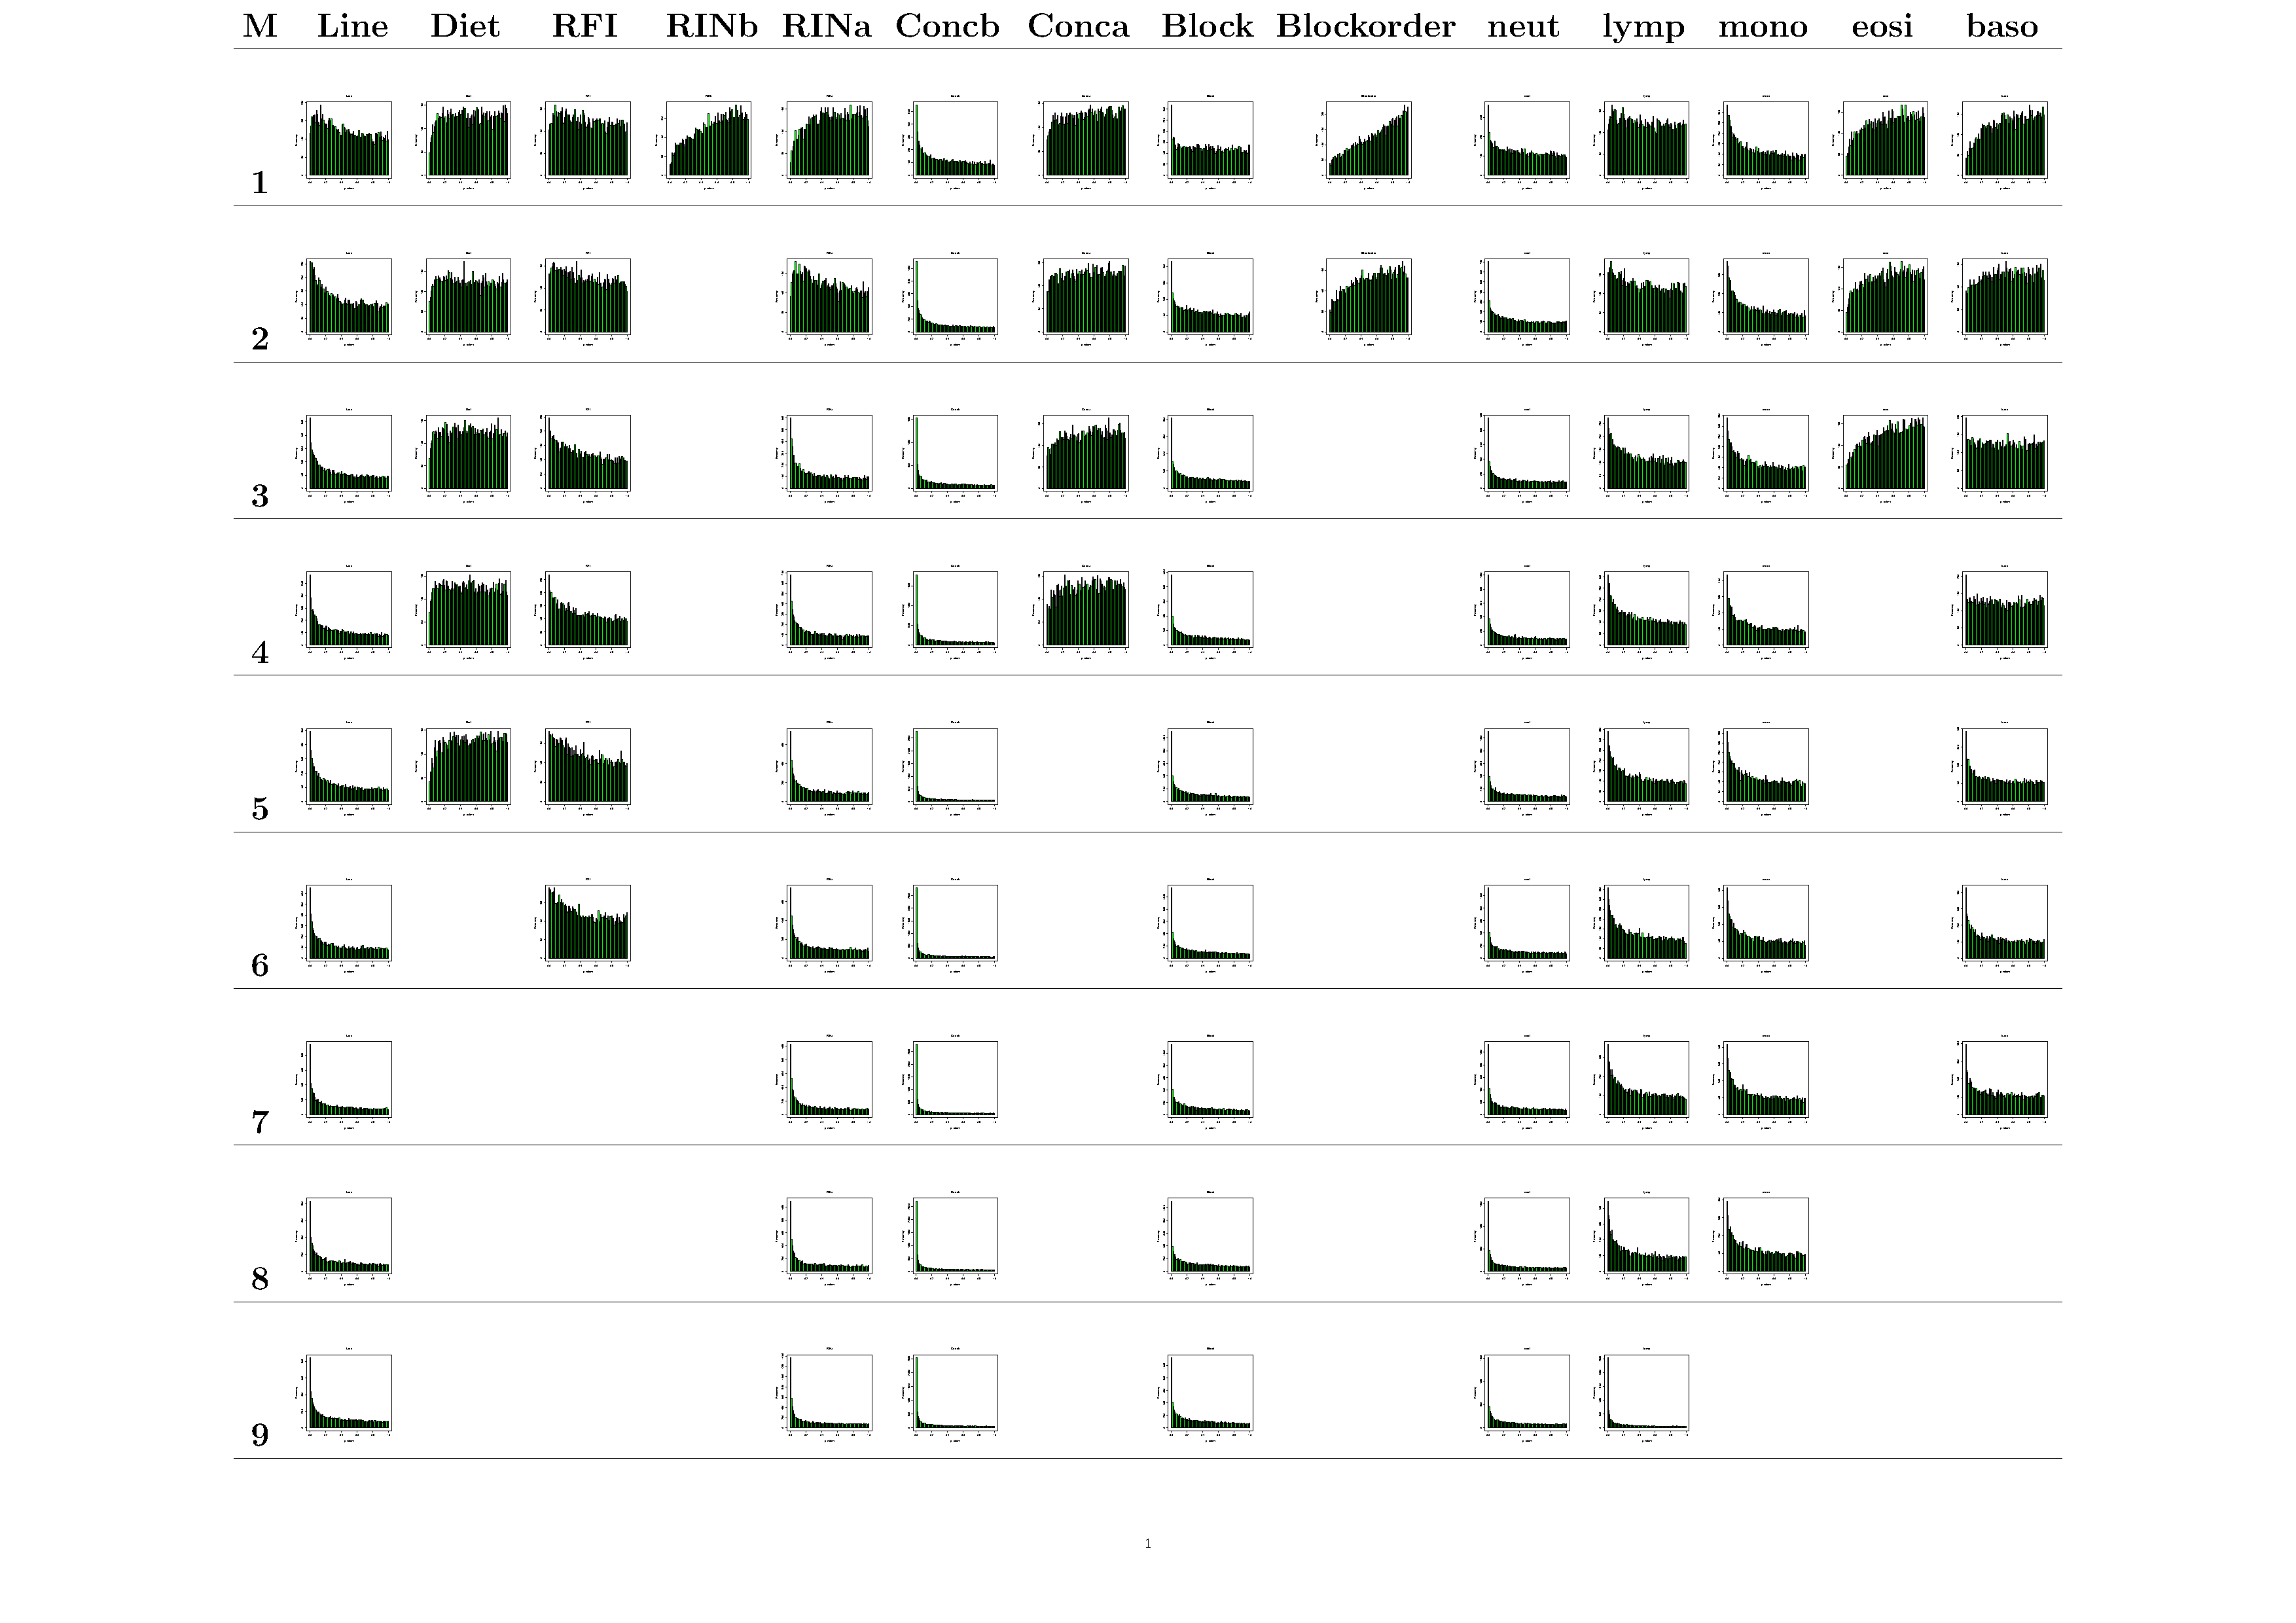
\includegraphics[scale = 0.27]{PlotG9P2PairedEndCBCpvalue05.pdf}
\caption{Backward Modelselection for RFI data using the criterion based on number of pvalue less than 0.05 in each step of excluding one covariate. }
\end{figure}


\begin{figure}[h!]
\centering
\includegraphics[scale = 0.27]{PlotG9P2PairedEndCBCks.pdf}
\caption{Backward Modelselection for RFI data using the criterion based on Kolmogorov-Smirnov statistics in each step of excluding one covariate. }
\end{figure}


\section{\bf Simulation Justification based on Real Data}
We perform a simulation study based on the RNASeq data from RFI project. From choosen 
model (model 7 of pvalue05 criterion), we obtain estimates of coeficients of $\beta_{Line}$ and $\beta$, also estimate of the number of true null $m_{0}$ for Line effect. Then we assign the coefficient $\beta_{Line}$ of  $m_0$  least significant genes (with respect to Line effect) = 0. The other coefficients keep the same. 

Next, we select the genes whose correlation of fitted count and real count data is at lest 0.8 to be the set of genes that we will simulate the count data. We randomly pickup 5000 genes from this set and simulate a count data of size $5000\times 31$ where each count value is simulated from a negative binomial distribution with mean and dispersion parameters are those of fitted original genes. Then, we apply pvalue05 criteria for selection model procedure. And we also run a model with only Line effect to do comparision. There are 100 simulations. The result is summarized in the table below.
% \begin{tabular}
% Method    & FDR(sdFDR)  & Rt (sdRt)\\
% pvalue05  & 0.105(0.002) &  
% \end{tabular}

% latex table generated in R 3.1.1 by xtable 1.7-3 package
% Mon Dec 01 12:06:59 2014
\begin{table}[ht]
\centering
{\scriptsize
\begin{tabular}{|c|cccccccccccccc|c|}
  \hline
$\pi$ & Line & Diet & RFI & Concb & RINb & Conca & RINa & neut & lymp & mono & eosi & baso & Block & Order & pvalue05 \\ 
  \hline
0.9 & 1 & 0 & 0 & 1 & 0 & 1 & 1 & 1 & 1 & 1 & 0 & 1 & 1 & 0 & 3 \\ 
  0.9 & 1 & 0 & 0 & 1 & 0 & 1 & 1 & 1 & 1 & 1 & 1 & 1 & 1 & 0 & 1 \\ 
  0.9 & 1 & 0 & 0 & 1 & 0 & 0 & 1 & 1 & 1 & 1 & 0 & 1 & 1 & 0 & 74 \\ 
  0.9 & 1 & 0 & 0 & 1 & 0 & 0 & 1 & 1 & 1 & 1 & 1 & 1 & 1 & 0 & 9 \\ 
  0.9 & 1 & 0 & 0 & 1 & 1 & 1 & 1 & 1 & 1 & 1 & 0 & 1 & 1 & 0 & 1 \\ 
  0.9 & 1 & 0 & 0 & 1 & 1 & 0 & 1 & 1 & 1 & 1 & 0 & 1 & 1 & 0 & 4 \\ 
  0.9 & 1 & 0 & 0 & 1 & 1 & 0 & 1 & 1 & 1 & 1 & 1 & 1 & 1 & 0 & 1 \\ 
  0.9 & 1 & 1 & 0 & 1 & 0 & 1 & 1 & 1 & 1 & 1 & 1 & 1 & 1 & 0 & 1 \\ 
  0.9 & 1 & 1 & 0 & 1 & 0 & 0 & 1 & 1 & 1 & 1 & 1 & 1 & 1 & 0 & 4 \\ 
  0.9 & 1 & 1 & 0 & 1 & 1 & 1 & 1 & 1 & 1 & 1 & 1 & 1 & 1 & 0 & 1 \\ 
  0.9 & 1 & 1 & 1 & 1 & 0 & 0 & 1 & 1 & 1 & 1 & 0 & 1 & 1 & 0 & 1 \\ 
   \hline
0.8 & 1 & 0 & 0 & 1 & 0 & 1 & 1 & 1 & 1 & 1 & 0 & 1 & 1 & 0 & 2 \\ 
  0.8 & 1 & 0 & 0 & 1 & 0 & 0 & 1 & 1 & 1 & 1 & 0 & 1 & 1 & 0 & 74 \\ 
  0.8 & 1 & 0 & 0 & 1 & 0 & 0 & 1 & 1 & 1 & 1 & 1 & 1 & 1 & 0 & 5 \\ 
  0.8 & 1 & 0 & 0 & 1 & 1 & 1 & 1 & 1 & 1 & 1 & 0 & 1 & 1 & 0 & 2 \\ 
  0.8 & 1 & 0 & 0 & 1 & 1 & 0 & 1 & 1 & 1 & 1 & 0 & 1 & 1 & 0 & 5 \\ 
  0.8 & 1 & 0 & 0 & 1 & 1 & 0 & 1 & 1 & 1 & 1 & 1 & 1 & 1 & 0 & 1 \\ 
  0.8 & 1 & 1 & 0 & 1 & 0 & 1 & 1 & 1 & 1 & 1 & 0 & 1 & 1 & 0 & 1 \\ 
  0.8 & 1 & 1 & 0 & 1 & 0 & 0 & 1 & 1 & 1 & 1 & 0 & 1 & 1 & 0 & 7 \\ 
  0.8 & 1 & 1 & 0 & 1 & 0 & 0 & 1 & 1 & 1 & 1 & 1 & 1 & 1 & 0 & 3 \\ 
   \hline
0.7 & 1 & 0 & 0 & 1 & 0 & 1 & 1 & 1 & 1 & 1 & 0 & 1 & 1 & 0 & 2 \\ 
  0.7 & 1 & 0 & 0 & 1 & 0 & 0 & 1 & 1 & 1 & 1 & 0 & 1 & 1 & 0 & 78 \\ 
  0.7 & 1 & 0 & 0 & 1 & 0 & 0 & 1 & 1 & 1 & 1 & 1 & 1 & 1 & 0 & 10 \\ 
  0.7 & 1 & 0 & 0 & 1 & 1 & 0 & 1 & 1 & 1 & 1 & 0 & 1 & 1 & 0 & 3 \\ 
  0.7 & 1 & 0 & 0 & 1 & 1 & 0 & 1 & 1 & 1 & 1 & 1 & 1 & 1 & 0 & 1 \\ 
  0.7 & 1 & 1 & 0 & 1 & 0 & 0 & 1 & 1 & 1 & 1 & 0 & 1 & 1 & 0 & 5 \\ 
  0.7 & 1 & 1 & 0 & 1 & 1 & 0 & 1 & 1 & 1 & 1 & 1 & 1 & 1 & 0 & 1 \\ 
   \hline
0.6 & 1 & 0 & 0 & 1 & 0 & 1 & 1 & 1 & 1 & 1 & 0 & 1 & 1 & 0 & 2 \\ 
  0.6 & 1 & 0 & 0 & 1 & 0 & 0 & 1 & 1 & 1 & 0 & 0 & 1 & 1 & 0 & 1 \\ 
  0.6 & 1 & 0 & 0 & 1 & 0 & 0 & 1 & 1 & 1 & 1 & 0 & 1 & 1 & 0 & 78 \\ 
  0.6 & 1 & 0 & 0 & 1 & 0 & 0 & 1 & 1 & 1 & 1 & 1 & 1 & 1 & 0 & 9 \\ 
  0.6 & 1 & 0 & 0 & 1 & 1 & 0 & 1 & 1 & 1 & 1 & 1 & 1 & 1 & 0 & 1 \\ 
  0.6 & 1 & 1 & 0 & 1 & 0 & 0 & 1 & 1 & 1 & 1 & 0 & 1 & 1 & 0 & 6 \\ 
  0.6 & 1 & 1 & 0 & 1 & 0 & 0 & 1 & 1 & 1 & 1 & 1 & 1 & 1 & 0 & 1 \\ 
  0.6 & 1 & 1 & 0 & 1 & 1 & 1 & 1 & 1 & 1 & 1 & 0 & 1 & 1 & 0 & 1 \\ 
  0.6 & 1 & 1 & 0 & 1 & 1 & 1 & 1 & 1 & 1 & 1 & 1 & 1 & 1 & 0 & 1 \\ 
   \hline
\end{tabular}
}
\end{table}
% latex table generated in R 3.1.1 by xtable 1.7-3 package
% Mon Dec 01 12:07:08 2014
\begin{table}[ht]
\centering
{\scriptsize
\begin{tabular}{|c|cccccccccccccc|c|}
  \hline
$\pi$ & Line & Diet & RFI & Concb & RINb & Conca & RINa & neut & lymp & mono & eosi & baso & Block & Order & ks \\ 
  \hline
0.9 & 1 & 0 & 0 & 1 & 0 & 1 & 1 & 1 & 1 & 1 & 1 & 1 & 1 & 0 & 1 \\ 
  0.9 & 1 & 0 & 0 & 1 & 0 & 0 & 1 & 1 & 1 & 1 & 0 & 1 & 1 & 0 & 69 \\ 
  0.9 & 1 & 0 & 0 & 1 & 0 & 0 & 1 & 1 & 1 & 1 & 0 & 1 & 1 & 1 & 4 \\ 
  0.9 & 1 & 0 & 0 & 1 & 0 & 0 & 1 & 1 & 1 & 1 & 1 & 1 & 1 & 0 & 9 \\ 
  0.9 & 1 & 0 & 0 & 1 & 1 & 0 & 1 & 1 & 1 & 1 & 0 & 1 & 1 & 0 & 6 \\ 
  0.9 & 1 & 1 & 0 & 1 & 0 & 1 & 1 & 1 & 1 & 1 & 1 & 1 & 1 & 0 & 2 \\ 
  0.9 & 1 & 1 & 0 & 1 & 0 & 0 & 1 & 1 & 1 & 1 & 0 & 1 & 1 & 0 & 1 \\ 
  0.9 & 1 & 1 & 0 & 1 & 0 & 0 & 1 & 1 & 1 & 1 & 1 & 1 & 1 & 0 & 2 \\ 
  0.9 & 1 & 1 & 0 & 1 & 1 & 1 & 1 & 1 & 1 & 1 & 1 & 1 & 1 & 0 & 1 \\ 
  0.9 & 1 & 1 & 0 & 1 & 1 & 0 & 1 & 1 & 1 & 1 & 0 & 1 & 1 & 0 & 1 \\ 
  0.9 & 1 & 1 & 1 & 1 & 1 & 1 & 1 & 1 & 1 & 1 & 0 & 1 & 1 & 0 & 1 \\ 
  0.9 & 1 & 1 & 1 & 1 & 1 & 1 & 1 & 1 & 1 & 1 & 1 & 1 & 1 & 1 & 3 \\ 
   \hline
0.8 & 1 & 0 & 0 & 1 & 0 & 1 & 1 & 1 & 1 & 1 & 0 & 1 & 1 & 0 & 2 \\ 
  0.8 & 1 & 0 & 0 & 1 & 0 & 1 & 1 & 1 & 1 & 1 & 1 & 1 & 1 & 0 & 1 \\ 
  0.8 & 1 & 0 & 0 & 1 & 0 & 0 & 1 & 1 & 1 & 1 & 0 & 1 & 1 & 0 & 77 \\ 
  0.8 & 1 & 0 & 0 & 1 & 0 & 0 & 1 & 1 & 1 & 1 & 1 & 1 & 1 & 0 & 7 \\ 
  0.8 & 1 & 0 & 0 & 1 & 1 & 0 & 1 & 1 & 1 & 1 & 0 & 1 & 1 & 0 & 2 \\ 
  0.8 & 1 & 0 & 0 & 1 & 1 & 0 & 1 & 1 & 1 & 1 & 1 & 1 & 1 & 0 & 1 \\ 
  0.8 & 1 & 1 & 0 & 1 & 0 & 0 & 1 & 1 & 1 & 1 & 0 & 1 & 1 & 0 & 7 \\ 
  0.8 & 1 & 1 & 0 & 1 & 0 & 0 & 1 & 1 & 1 & 1 & 1 & 1 & 1 & 0 & 1 \\ 
  0.8 & 1 & 1 & 1 & 1 & 1 & 1 & 1 & 1 & 1 & 1 & 1 & 1 & 1 & 1 & 2 \\ 
   \hline
0.7 & 1 & 0 & 0 & 1 & 0 & 1 & 1 & 1 & 1 & 1 & 0 & 1 & 1 & 0 & 2 \\ 
  0.7 & 1 & 0 & 0 & 1 & 0 & 0 & 1 & 1 & 1 & 1 & 0 & 1 & 1 & 0 & 79 \\ 
  0.7 & 1 & 0 & 0 & 1 & 0 & 0 & 1 & 1 & 1 & 1 & 1 & 1 & 1 & 0 & 8 \\ 
  0.7 & 1 & 0 & 0 & 1 & 1 & 0 & 1 & 1 & 1 & 1 & 0 & 1 & 1 & 0 & 2 \\ 
  0.7 & 1 & 0 & 0 & 1 & 1 & 0 & 1 & 1 & 1 & 1 & 1 & 1 & 1 & 0 & 2 \\ 
  0.7 & 1 & 1 & 0 & 1 & 0 & 0 & 1 & 1 & 1 & 1 & 0 & 1 & 1 & 0 & 4 \\ 
  0.7 & 1 & 1 & 0 & 1 & 0 & 0 & 1 & 1 & 1 & 1 & 1 & 1 & 1 & 0 & 2 \\ 
  0.7 & 1 & 1 & 0 & 1 & 1 & 0 & 1 & 1 & 1 & 1 & 1 & 1 & 1 & 0 & 1 \\ 
   \hline
0.6 & 1 & 0 & 0 & 1 & 0 & 1 & 1 & 1 & 1 & 1 & 0 & 1 & 1 & 0 & 1 \\ 
  0.6 & 1 & 0 & 0 & 1 & 0 & 0 & 1 & 1 & 1 & 1 & 0 & 1 & 1 & 0 & 82 \\ 
  0.6 & 1 & 0 & 0 & 1 & 0 & 0 & 1 & 1 & 1 & 1 & 1 & 1 & 1 & 0 & 8 \\ 
  0.6 & 1 & 0 & 0 & 1 & 1 & 0 & 1 & 1 & 1 & 1 & 0 & 1 & 1 & 0 & 1 \\ 
  0.6 & 1 & 1 & 0 & 1 & 0 & 0 & 1 & 1 & 1 & 1 & 0 & 1 & 1 & 0 & 4 \\ 
  0.6 & 1 & 1 & 0 & 1 & 0 & 0 & 1 & 1 & 1 & 1 & 1 & 1 & 1 & 0 & 3 \\ 
  0.6 & 1 & 1 & 0 & 1 & 1 & 1 & 1 & 1 & 1 & 1 & 0 & 1 & 1 & 0 & 1 \\ 
   \hline
\end{tabular}
}
\end{table}


\newpage

\begin{knitrout}
\definecolor{shadecolor}{rgb}{0.969, 0.969, 0.969}\color{fgcolor}

{\centering \includegraphics[width=\maxwidth]{figure/minimal-unnamed-chunk-3} 

}



\end{knitrout}

\section*{Acknowledgments}
% This material is based upon work supported by Agriculture and Food
% Research Initiative Competitive Grant No. 2011-68004-30336 from
% the USDA National Institute of Food and Agriculture, and the
% National Science Foundation (NSF) under Grant No. 0922746.
% Any opinions, findings, and conclusions or recommendations expressed
% in this material are those of the authors and do not necessarily reflect
% the views of the USDA or NSF.

%% HERE WE DECLARE THE BIBLIOGRAPHYSTYLE TO USE AND THE BIBLIOGRAPHY DATABASE

\end{document}
